\documentclass[11pt]{article}
\usepackage{a4, fullpage}
\usepackage{bibtopic}
\usepackage[small,compact]{titlesec}
\usepackage{float}
\usepackage{amssymb,amsmath}
\usepackage[T1]{fontenc}
\usepackage{graphicx}
\usepackage{multicol}
\usepackage{multirow}
\usepackage{listings}
\usepackage{pdfpages}
\usepackage{booktabs}

\restylefloat{table}

%\setlength{\parskip}{0.3cm}
%\setlength{\parindent}{0cm}
%\setlength{\textheight}{10.7in} %used to be 10
%\setlength{\textwidth}{6.5in}
%\setlength{\parskip}{2pt}
%\addtolength{\oddsidemargin}{-.3in}
%\addtolength{\evensidemargin}{-.3in}
%\addtolength{\topmargin}{-.6in}
%\addtolength{\textwidth}{.6in}


\begin{document}

\title{\vspace{100px} BUSINESS PLAN \\ \vspace{100px} Shimla Gold Cider \vspace{100px}}
%\author{\vspace{50px}John Walker, Rutwik Shah, Sahil Jain, Alina Boghiu, Giovanni Charles, Łukasz Koprowski \vspace{50px}}

%Imperial College London, Department of Computing

\date{\today}         % inserts today's date

\maketitle           % generates the title from the data above

\newpage

\title{ \hspace{100px} SHIMLA GOLD CIDER BUSINESS PLAN}
\maketitle

\begin{table}[H]
\begin{center}
\begin{tabular}{| p{7cm} | p{7cm} |}
\hline
Date Stamp of this Document:     &  \today  \\
\hline
Version of this Document:        &  V.0.2  \\
\hline
Author/Editor of this Document:  & Adam Fiksen, \newline Alina Boghiu, \newline Giovanni Charles, \newline John Walker, \newline Rutwik Shah, \newline Sahil Jain, \newline Lukaz Koprowski  \\
\hline
\end{tabular}
\end{center}
\end{table}

\title{ \hspace{175px} DISCLAIMER \\}
\maketitle

\noindent This business plan has been prepared by the authors and is being provided to a limited number of
persons, at their request.This document is confidential and is only being made available to
parties who agree to keep it confidential.Neither this business plan nor any part of it shall be
copied, reproduced or distributed to others at any time without the prior written consent of the authors.
By accepting this document the recipient is deemed to undertake and warrant to the authors that the
recipient will keep it confidential and that the recipient shall return all copies of this document
to the authors immediately upon request. \\

\noindent Although X has taken reasonable care to ensure that the information contained in this
document is accurate, no other representation or warranty, express or implied, is or will be
given by X or any of its agents.No responsibility is or will be accepted by the authors or any of its
agents as to the accuracy or completeness of this document or the information or opinions
contained herein.Recipients must make their own investigations and must satisfy themselves
as to the condition and prospects of the authors and the accuracy and completeness of statements
contained herein. \\

\noindent Any financial projections given in this plan are illustrative only.Because of the early stage
nature of the authors’ business, none of the projections given in this document should be taken as
guaranteed to be attainable, nor should they be taken as implying any indication, assurance
or guarantee that those assumptions are correct or exhaustive.


\begin{table}[H]
\begin{center}
\begin{tabular}{|p{7cm}  p{7cm} |}
\hline
Issued To:      & Nick Coutts         \\
Company:        &  Shimla Gold Cider  \\
Date of Issue:  &  \today            \\
Copy Number:    &  1                  \\
\hline
\end{tabular}
\end{center}
\end{table}

\newpage

\tableofcontents


%------------------------EXECUTIVE SUMMARY-------------------------------------%
\section{Executive Summary}
  \subsection{Overview}
  %A patented solution...
  %Vision to be...
  %Consumer and regulatory pressure...
  %Has clear competitve advantages...
  %Has unsurpassed technology and has sales through...
  \subsection{Market Drivers}
  %Market drivers....
  \subsection{Business Proposition}
  %Meets increasing demands...
  \subsection{Financial Summary and Investment Proposition}
  %Requires...
%------------------------------------------------------------------------------%
%------------------------MARKET OPPORTUNITY------------------------------------%
\section{Market Opportunity}
  \subsection{The Opportunity for Shimla Gold Cider}
  %Addressable market of...  
  \subsection{Market Segments}
  %Clear market segments Including...
%------------------------------------------------------------------------------%
%------------------------PRODUCT PROPOSITION-----------------------------------%
\section{Shimla Gold Cider Product Proposition}
%Has superior technology in....
  \subsection{Shimla Gold Cider's Unique Proposition}
  %Is proven cost effective and easy to implement...
  \subsection{Business Model}
  \newpage
  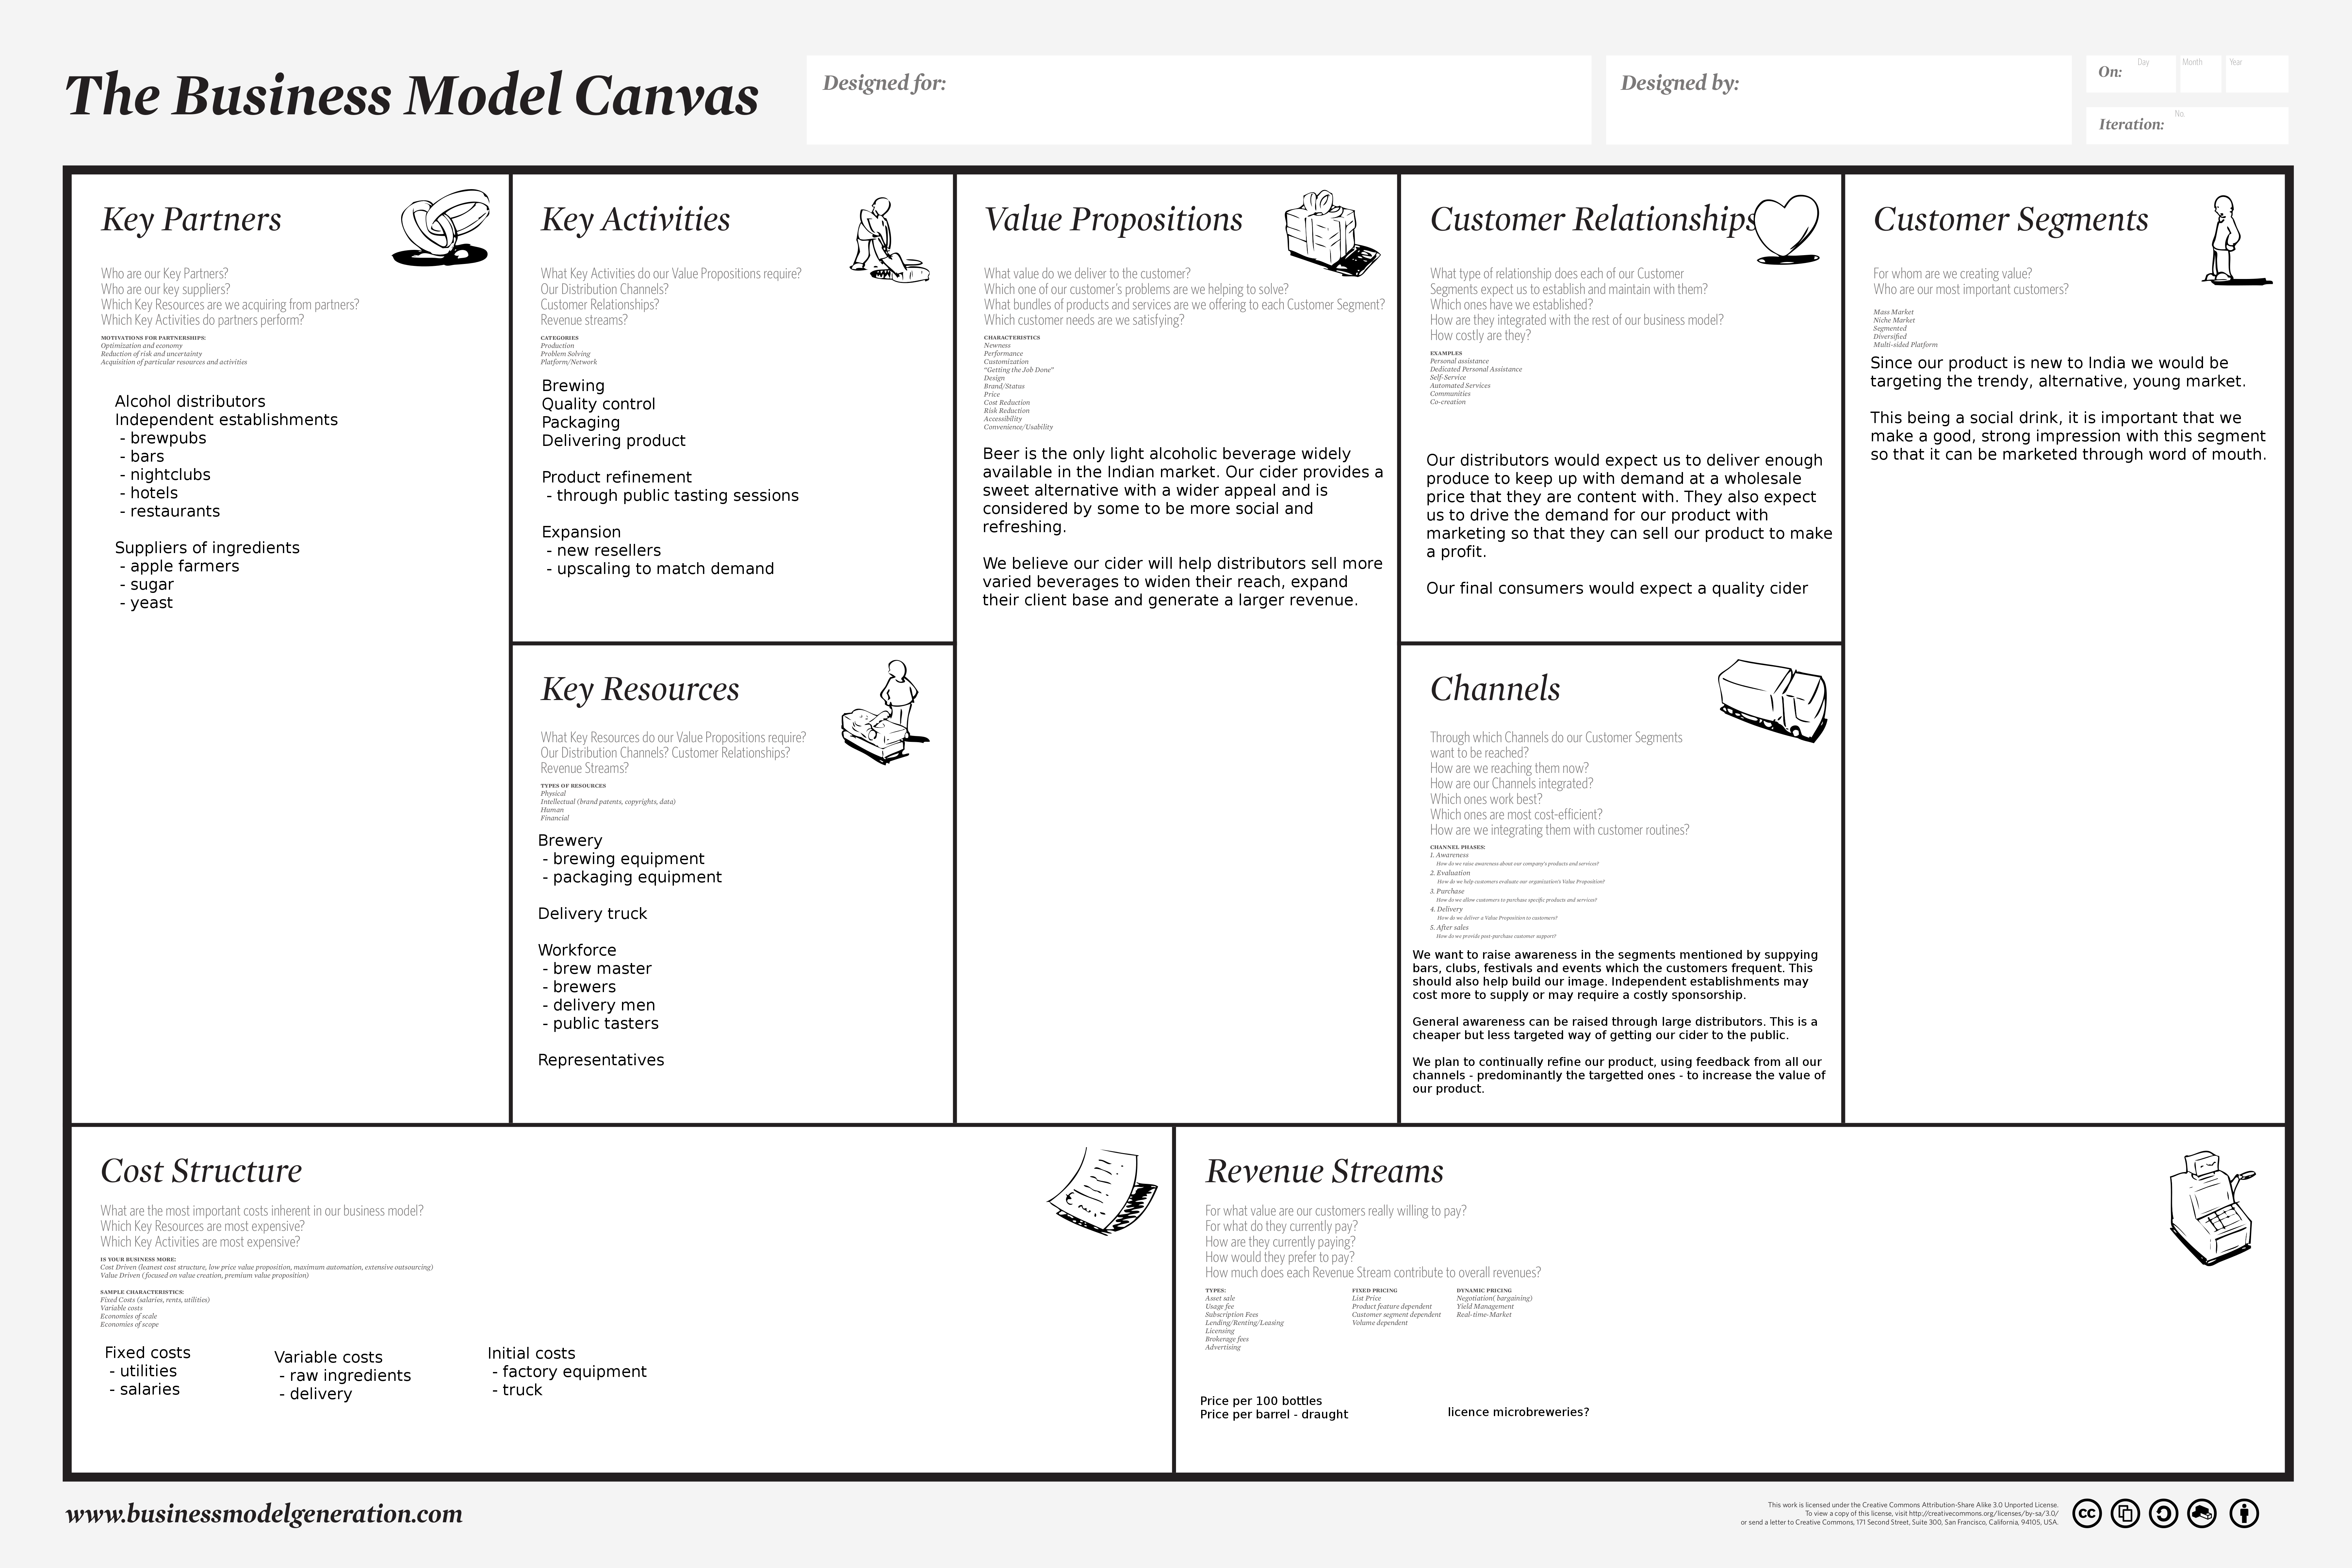
\includegraphics[angle=90,width=\textwidth,height=\textheight,keepaspectratio]{./business_model_canvas_poster.png}
   %Established production, sales & marketing, distibution model...
%------------------------------------------------------------------------------%
%------------------------TARGET MARKET-----------------------------------------%
\section{Target Market}
  \subsection{Market Context}
  %Global vision well defined market segments and territories...
  \subsection{Market Size and Characteristics}
  %This equates to a global revenue opportunity of??? 
  %Diagram yearly market potential
  \subsection{Market Validation}
  %Has met all technical norms
%------------------------------------------------------------------------------%
%------------------------MARKET DEVELOPMENT PLAN-------------------------------%
\section{Market Development Plan}
  \subsection{Sales Process}
  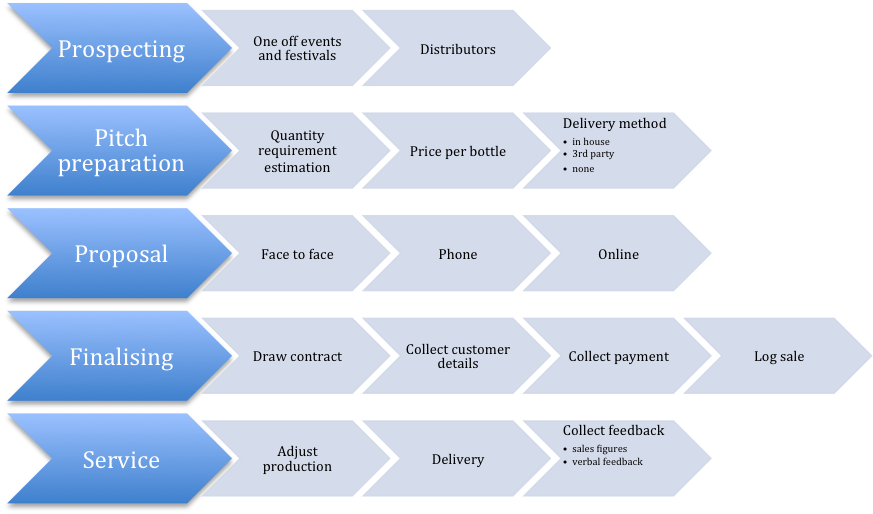
\includegraphics[width=\textwidth,keepaspectratio]{./process.png}
  %Proven sales process...
  %Good relationship with strong distributor...
  \subsection{Target Customers}
  %Larger customers as targets
  \subsection{Current Key Customers}
  %Large current customers
  \subsection{Marketing, PR and Communications}
We aim at advertising at horse racing events this has a cost of Rs. 5,00,000 though this number is high it has several benefits in doing so:
\begin{itemize}
\item 1) Conduct contests of skill and award prizes to the public to generate interest. 
\item 2) Advertise on the CCTV transmission at all centers .
\item 3) Have full rights for on-site branding across the stands.
\item 4) Name the race to suit its preference.
\item 5) Have its CEO / nominee present the trophy.
\item 6) Be entitled to the free use of lawns above a certain value of sponsorship.
\item 7) Arrange for live entertainment at race time or before or after the event.
\item 8) Promote and your brand the race via mailers/press.
\item 9) Have access to the Club's membership data which consists of thousands of potential customers who represent some of the most well off clients in India.
\item 10) Have promotion on the website with links to the lounges webpage.
\item 11) Get coverage on a major television network as these races will be viewed world wide.

\end{itemize}
%------------------------------------------------------------------------------%
%------------------------COMPETITION-------------------------------------------%
\section{Competition}
%Limited number of direct competitors
  \subsection{Competitive Advantage}
  %Competitve advantage in technology
%------------------------------------------------------------------------------%
%------------------------INTELLECTUAL PROPERTY (IP) ASSETS---------------------%
\section{Intellectual Property (IP) Assets}
  \subsection{Shimla Gold Cider Solution}
    \subsubsection{Patents}
    %Technology protected 1. 2. 3. ....
    \subsubsection{Know-How}
    %Internation experts choose to work with X
  \subsection{Future IP Developments}
  %Future applications plannes along with IP Protection...
%------------------------------------------------------------------------------%
%------------------------BUSINESS GROWTH AND RESOURCE PLANS--------------------%
\section{Business Growth and Resource Plans}
  \subsection{Current Structure and Resources}
  %Early phase centred on technology development
  \subsection{Straff Recruitment}

The average cost of hiring for the skilled workers is about Rs. 1,00,000 a year we would require :
\begin{itemize}

\item 2 workers in charge of apple receival, washing and sorting  
\item 1 worker in charge of general cleaning of the area
\item 2 workers in charge of apple grating
\item 2 workers in charge of apple pressing
\item 2 workers in charge of apple pressing 

\end{itemize}

Further as required we will require a security guard which will cost about Rs. 50,000 a year.
 
  \subsection{Facilities}
Since we aim at setting up a microbrewery to start with in at a manufacturing area in Himachal Pradesh

Rent in this area is roughly about Rs.1 / ft$^2$ per month.
As seen in the requirements:

there is a storage area required this has been estimated to: 500 sq $^2$
area of for manufacturing the product would be 1500 ft$^2$ this is plenty to space to meet estimated current requirements

Lunch area and office space is estimated to be about 1000 $^2$ as well this as above well allows some space for hiring a few more employees if and when needed.

Hence yearly rent works out at Rs. 24,000 per year.
%------------------------------------------------------------------------------%
%------------------------FINANCIAL PLAN AND FUNDING ASSUMPTIONS----------------%
\section{Financial Plan and Funding Assumptions}
  \subsection{Financial History}
  \subsection{Financial Projections}
  \subsection{Use of Funds}
   
cost of sugar -  Rs.30 / kg
campden tables  - Rs.300 per 100 tablets
Sweet mead Rs.500 for /128 gms 


This bring the cost of dry cider to Rs. 5.866 per 330 ml
This bring the sweet of dry cider to Rs. 6.4 per 330 ml
  %Funds needed for sales and marketing support
%------------------------------------------------------------------------------%
%------------------------EXIT STRATEGY-----------------------------------------%
\section{Exit Strategy}
%Exit-trade sale
%------------------------------------------------------------------------------%
%------------------------RISK ANALYSIS-----------------------------------------%
\section{Risk Analysis}
  \subsection{Risk Assessment and Management}
   %Strong distribution channels minimise risk as does IP protection
%------------------------------------------------------------------------------%
%------------------------COMPANY STRUCTURE AND MANAGEMENT PROFILES-------------%
\section{Company Structure and Management Profiles}
  \subsection{Current Equity Structure}
  %Clear ownership structure
  \subsection{Management Team}
  %Expirences management team
  \subsection{Corporate Information}
  %Directors
  %Registered Number
  %Registered Office
  %VAT Number
  %Company Auditors
  %Company Lawyers
  %Company Bankers
  \subsection{Location and Contact Details}
%------------------------------------------------------------------------------%
%------------------------ANNEX 1-----------------------------------------------%
\section{ANNEX 1}
%------------------------------------------------------------------------------%
%------------------------MARKET PLAYERS----------------------------------------%
\section{Market Players}
%------------------------------------------------------------------------------%
%------------------------ANNEX 2-----------------------------------------------%
\section{ANNEX 2}
%------------------------------------------------------------------------------%
%------------------------ANNEX 3-----------------------------------------------%
\section{ANNEX 3}
%------------------------------------------------------------------------------%
%------------------------COMPANY BACKGROUND------------------------------------%
\section{Company Background}
%------------------------------------------------------------------------------%

\end{document}
